
\section{\BookRecordIndex{T0257}粘合映射的满射性}\label{sec:10-7}

现在回到\BookRecordIndex{T0256}粘合定理的证明，完成最后一步，即证明定理~\ref{thm:10-1-2}
中关于满射性的第（v）部分\sourcefootnote{原书在本段把关于满射性的结论写成第（iv）部分；但紧接着
的证明标题、四个步骤及证明结尾均明确指向定理~\ref{thm:10-1-2} 的第（v）部分，故补正。}
的证明。困难在于，我们所考虑的 $J^R$-全纯曲线 $v$ 仅在很弱的意义下接近
$\mathcal M(c-1)$：只假设存在一对
$(u^0,u^\infty)\in\mathcal M(c-1)$，使得 $v$ 在圆盘 $\{|z|\geq1\}$ 上的限制
在 $C^0$ 意义下接近 $u^0$，而它在圆盘 $\{|z|\leq1/R^2\}$ 上的限制在
$C^0$ 意义下接近重标度 $u^\infty(R^2z)$。我们必须仅凭这些有限的信息证明
$v$ 位于 $\iota_c^R$ 的像中。尽管逆函数定理包含唯一性陈述，该陈述却很受限制：
它只在我们已经找到一个\BookRecordIndex{T0394}预粘合元素 $u^R$，使得
$v=\exp_{u^R}(\xi)$、$\xi$ 位于逆算子 $Q_{u^R}$ 的像中且在 $W^{1,p}$ 意义下
充分小时才适用。因此，我们用逐次逼近来证明满射性：先假设 $v$ 满足一个相当强的
条件，再依次考虑越来越弱的条件。

\begin{proof}[定理~\ref{thm:10-1-2} 第（v）部分的证明]
证明分为四步。

\medskip
\noindent\textbf{步骤 1.}
\emph{存在常数 $\varepsilon_1>0$，使得对每个
$(\delta,R)\in\mathcal A(\delta_0)$，下述结论成立。若
$u:=(u^0,u^\infty)\in\mathcal M(c)$、$u^R:=f^R(u)$ 以及
$\xi^R\in\Omega^0(S^2,(u^R)^*TM)$ 满足}
\[
  \xi^R\in\operatorname{im}Q_{u^R},\qquad
  \bar\partial_{J^R}\bigl(\exp_{u^R}(\xi^R)\bigr)=0,
  \qquad \lVert\xi^R\rVert_{1,p,R}<\varepsilon_1,
\]
\emph{则 $\exp_{u^R}(\xi^R)=\iota_c^R(u)$。}

由式~\eqref{eq:10-5-12} 中定义\BookRecordIndex{T0257}粘合映射 $\iota_c^R$ 之前的讨论，这立即来自
定理~\ref{thm:3-5-2} 的唯一性结论，其中取
$u=u^R$、$\xi_0=0$、$\xi=\xi^R$。（关于依赖于 $z$ 的\BookRecordIndex{T0088}殆复结构，见
注~\ref{rem:3-5-4}。）

\medskip
\noindent\textbf{步骤 2.}
\emph{对每个 $\varepsilon_1>0$，存在正常数 $\delta_2$ 和 $\varepsilon_2$，
使得对每个 $(\delta,R)\in\mathcal A(\delta_2)$，下述结论成立。若
$u:=(u^0,u^\infty)\in\mathcal M(c-1)$、$u^R:=f^R(u)$ 以及
$\xi^R\in\Omega^0(S^2,(u^R)^*TM)$ 满足}
\begin{equation}\label{eq:10-7-1}
  v:=\exp_{u^R}(\xi^R)\in\mathcal M(A;J^R),
  \qquad \lVert\xi^R\rVert_{1,p,R}<\varepsilon_2,
\end{equation}
\emph{则存在一对 $\bar u:=(\bar u^0,\bar u^\infty)\in\mathcal M(c)$，以及沿
$\bar u^R:=f^R(\bar u)$ 的向量场
$\bar\xi^R\in\Omega^0(S^2,(\bar u^R)^*TM)$，使得}
\begin{equation}\label{eq:10-7-2}
  v=\exp_{\bar u^R}(\bar\xi^R),\qquad
  \bar\xi^R\in\operatorname{im}Q_{\bar u^R},\qquad
  \lVert\bar\xi^R\rVert_{1,p,R}\leq\varepsilon_1.
\end{equation}

固定 $(\delta,R)\in\mathcal A(\delta_0)$ 和 $v\in\mathcal M(A;J^R)$。
不妨假设 $c_0\varepsilon_1$ 小于 $M$ 关于任一度量 $g_{J_z^0}$ 和
$g_{J_z^\infty}$ 的\BookRecordIndex{T0093}单射半径。必要时，我们会在证明过程中进一步缩小
$\varepsilon_1$。记
\[
  \mathcal U_1\subset\mathcal M(c)
\]
为所有满足下述条件的偶对 $u:=(u^0,u^\infty)\in\mathcal M(c)$ 所成的集合：
存在某个向量场 $\xi^R=\xi^R(u)$，使得
\begin{equation}\label{eq:10-7-3}
  \exp_{u^R}(\xi^R)=v,\qquad
  \lVert\xi^R\rVert_{1,p,R}<\varepsilon_1.
\end{equation}
注意，由引理~\ref{lem:10-3-1}，
$\lVert\xi^R\rVert_{L^\infty}\leq c_0\lVert\xi^R\rVert_{1,p,R}
\leq c_0\varepsilon_1$，所以这样的向量场 $\xi^R$ 至多有一个。

我们必须找到一个具有如下意义的常数 $\varepsilon_2>0$：若存在
$u\in\mathcal U_1$ 使 $\lVert\xi^R(u)\rVert_{1,p,R}<\varepsilon_2$，则存在
$\bar u:=(\bar u^0,\bar u^\infty)\in\mathcal U_1$，使相应的向量场
\[
  \bar\xi^R:=\xi^R(\bar u)
  \in\Omega^0(S^2,(\bar u^R)^*TM)
\]
属于算子 $Q_{\bar u^R}$ 的像。为证明这一点，先注意
$\mathcal M(c)$ 是维数为
\[
  m:=2n+2c_1(A)
\]
的光滑流形。由引理~\ref{lem:10-6-3}，当 $u\in\mathcal M(c)$、
$u^R:=f^R(u)$ 且 $R$ 充分大时，这也是 $D_{u^R}$ 的核的维数。

接着在 $u\in\mathcal U_1$ 上选取光滑\BookRecordIndex{T0067}标架
\[
  u\longmapsto\Xi_i(u)\in\ker D_u,
  \qquad D_u:=D_{u^0,u^\infty},
  \qquad i=1,\ldots,m.
\]
当 $\varepsilon_1$ 充分小且 $\delta R$ 充分大时，这样的\BookRecordIndex{T0067}标架存在，因为此时
$\mathcal U_1$ 包含于 $\mathcal M(c)$ 的一个坐标卡中。定义
\[
  \Xi_i^R(u):=
  \bigl(\mathbf 1-Q_{u^R}D_{u^R}\bigr)df^R(u)\Xi_i(u),
  \qquad i=1,\ldots,m.
\]
我们证明，当 $\delta R$ 充分大时，这是 $u\in\mathcal U_1$ 上
$\ker D_{u^R}$ 的一个\BookRecordIndex{T0067}标架。事实上，由引理~\ref{lem:10-6-3}，当 $\delta R$
充分大时，线性映射
\[
  \bigl(\mathbf 1-Q_{u^R}D_{u^R}\bigr)df^R(u):
  \ker D_u\longrightarrow\ker D_{u^R}
\]
对 $u\in\mathcal U_1$ 和 $u^R:=f^R(u)$ 是同构，而且其逆有一致界。因此存在
正常数 $c_3$ 和 $\delta_2$，使得只要
$(\delta,R)\in\mathcal A(\delta_2)$，对每个 $u\in\mathcal U_1$ 和
$y=(y_1,\ldots,y_m)\in\mathbb R^m$ 都有
\begin{equation}\label{eq:10-7-4}
  |y|\leq c_3
  \left\lVert\sum_{i=1}^m y_i\Xi_i^R(u)\right\rVert_{1,p,R}.
\end{equation}
所以，正如所断言的，$u\mapsto(\Xi_i^R(u))_{i=1}^m$ 是一个\BookRecordIndex{T0067}标架。
必要时增大 $c_3$，还可以使 $\mathcal U_1$ 中每条光滑道路
$t\mapsto u_t$ 满足
\begin{equation}\label{eq:10-7-5}
  \bigl\lVert\nabla_t\Xi_i^R(u_t)\bigr\rVert_{1,p,R}
  \leq c_3\lVert\partial_tu_t\rVert_{L^2},
  \qquad i=1,\ldots,m.
\end{equation}
为说明这一点，先设
$\xi_t=(\xi_t^0,\xi_t^\infty)\in T_{u_t}\mathcal M(c)$ 是沿 $u_t$ 的任意
光滑向量场。于是 $\nabla_t(df^R(u_t)\xi_t)$ 的 $(1,p,R)$-范数可由
\[
  C\bigl(\lVert\nabla_t\xi_t\rVert_{W^{1,p}}
  +\lVert\xi_t\rVert_{W^{1,p}}
   \lVert\partial_tu\rVert_{W^{1,p}}\bigr)
\]
估计。把这个不等式用于 $\xi_t:=\Xi_i(u_t)$，再使用
引理~\ref{lem:10-6-2} 和式~\eqref{eq:10-6-8}，即得
式~\eqref{eq:10-7-5}。（类似的论证见下面式~\eqref{eq:10-7-9} 的证明。）

\begin{figure}[tbp]
\centering
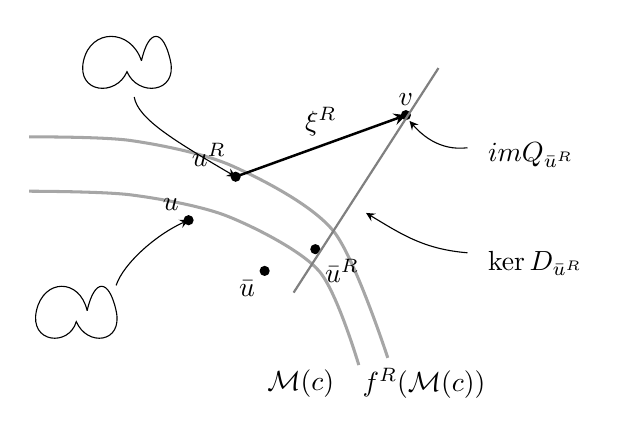
\begin{tikzpicture}[>=stealth,scale=.92]
  \draw[gray!70,line width=1.1pt]
    plot[smooth] coordinates {(-4.2,1.5) (-2.8,1.45) (-1.4,1.1) (0,.2) (.75,-1.55)};
  \draw[gray!70,line width=1.1pt]
    plot[smooth] coordinates {(-4.2,.75) (-2.8,.7) (-1.45,.4) (-.2,-.35) (.35,-1.65)};
  \node at (-.45,-1.9) {$\mathcal M(c)$};
  \node at (1.25,-1.9) {$f^R(\mathcal M(c))$};

  \coordinate (u) at (-2.0,.35);
  \coordinate (ub) at (-.95,-.35);
  \coordinate (uR) at (-1.35,.95);
  \coordinate (ubR) at (-.25,-.05);
  \coordinate (v) at (1.0,1.8);
  \fill (u) circle (2pt) node[above left] {$u$};
  \fill (ub) circle (2pt) node[below left] {$\bar u$};
  \fill (uR) circle (2pt) node[above left] {$u^R$};
  \fill (ubR) circle (2pt) node[below right] {$\bar u^R$};
  \fill (v) circle (2pt) node[above] {$v$};
  \draw[->,line width=.9pt] (uR) -- node[above] {$\xi^R$} (v);

  \draw[gray,line width=.8pt] (-.55,-.65) -- (1.45,2.45);
  \node[anchor=west] at (2.0,-.25) {$\ker D_{\bar u^R}$};
  \draw[->] (1.85,-.1) .. controls (1.25,-.05) and (.95,.15) .. (.45,.45);
  \node[anchor=west] at (2.0,1.25) {$\operatorname{im}Q_{\bar u^R}$};
  \draw[->] (1.85,1.35) .. controls (1.45,1.3) and (1.2,1.55) .. (1.05,1.72);

  \draw[thin] (-2.65,2.55) .. controls (-2.8,3.0) and (-3.35,3.0) .. (-3.45,2.55)
    .. controls (-3.55,2.1) and (-3.0,2.05) .. (-2.85,2.4)
    .. controls (-2.7,2.05) and (-2.15,2.1) .. (-2.25,2.55)
    .. controls (-2.35,3.0) and (-2.55,3.0) .. (-2.65,2.55);
  \draw[->] (-2.75,2.05) .. controls (-2.7,1.75) and (-2.2,1.45) .. (uR);
  \draw[thin] (-3.4,-.9) .. controls (-3.5,-.45) and (-4.0,-.45) .. (-4.1,-.9)
    .. controls (-4.2,-1.35) and (-3.65,-1.4) .. (-3.55,-1.05)
    .. controls (-3.4,-1.4) and (-2.9,-1.35) .. (-3.0,-.9)
    .. controls (-3.1,-.45) and (-3.3,-.45) .. (-3.4,-.9);
  \draw[->] (-3.0,-.55) .. controls (-2.9,-.25) and (-2.45,.15) .. (u);
\end{tikzpicture}
\caption{$f^R(\mathcal M(c))$ 的\BookRecordIndex{T0117}法丛。}\label{fig:10-7-2}
\end{figure}

定义光滑映射
\[
  h^R=(h_1^R,\ldots,h_m^R):\mathcal U_1\longrightarrow\mathbb R^m
\]
如下：
\begin{equation}\label{eq:10-7-6}
  \xi^R-Q_{u^R}D_{u^R}\xi^R
  =:\sum_{i=1}^m h_i^R(u)\Xi_i^R(u),
\end{equation}
其中 $u^R:=f^R(u)$，而 $\xi^R=\xi^R(u)$ 是沿 $u^R$、满足
式~\eqref{eq:10-7-3} 的唯一向量场。因此，$h^R(u)\in\mathbb R^m$ 是
$\xi^R(u)$ 沿 $Q_{u^R}$ 的像投影到 $D_{u^R}$ 的核后所得坐标向量。我们需要找到
一点 $\bar u$，使 $h^R(\bar u)$ 为零。由式~\eqref{eq:10-7-4}，存在常数
$c_4>0$，使得
\[
  |h^R(u)|\leq c_4\lVert\xi^R(u)\rVert_{1,p,R}.
\]
所以我们的假设蕴含：对某个可由我们选取的充分小 $\varepsilon_2$，存在
$u\in\mathcal U_1$ 使 $|h^R(u)|<c_4\varepsilon_2$。为找到 $h^R$ 的真正零点，
我们要应用命题 A.3.4。该命题是\BookRecordIndex{T0380}隐函数定理的一个版本：若映射 $h$ 在点 $x_1$ 有一个
近似零点，而且微分 $dh$ 在 $x_1$ 的一个充分大邻域上一致可逆，那么 $h$ 在非常靠近
$x_1$ 的地方有一个真正零点。

因此只须估计 $dh^R$ 的逆。其几何图像见图~\ref{fig:10-7-2}。向量
$\xi^R=\xi^R(u)$ 从 $u^R$ 指向 $v$。当 $u$ 沿切向量
$\dot u\in T_u\mathcal M(c)$ 的方向变化时，向量 $\xi^R\simeq v-u$ 大致沿
$-\dot u$ 的方向变化。由于 $h^R(u)$ 表示 $\xi^R(u)$ 到 $D_{u^R}$ 的核上的投影，
而该核几乎平行于 $D_u$ 的核，我们预期映射 $u\mapsto h^R(u)$ 的微分近似等于负恒等
映射；这里通过\BookRecordIndex{T0067}标架 $\Xi_1(u),\ldots,\Xi_m(u)$ 把
$T_u\mathcal M(c)$ 与 $\mathbb R^m$ 识别。下面把这一直观说法精确化。

记
\[
  H(u):=(H_1(u),\ldots,H_m(u)):\ker D_u\longrightarrow\mathbb R^m
\]
为\BookRecordIndex{T0067}标架 $\Xi_1(u),\ldots,\Xi_m(u)$ 所给出的同构，也就是说
\[
  \sum_{i=1}^m(H_i(u)\xi)\Xi_i(u)=\xi.
\]
于是，由 $\Xi_i^R(u)$ 的定义，对 $\xi\in\ker D_u=T_u\mathcal M(c)$ 有
\[
  \sum_{i=1}^m(H_i(u)\xi)\Xi_i^R(u)
  =\bigl(\mathbf 1-Q_{u^R}D_{u^R}\bigr)df^R(u)\xi.
\]
我们将证明存在常数 $c_5>0$，使得对每个
$u:=(u^0,u^\infty)\in\mathcal U_1$ 都有
\begin{equation}\label{eq:10-7-7}
  \lVert dh^R(u)+H(u)\rVert\leq c_5\varepsilon_1.
\end{equation}
这里 $\lVert\cdot\rVert$ 表示从 $\ker D_u$ 到 $\mathbb R^m$ 的线性映射的算子范数，
其中 $\mathbb R^m$ 取欧几里得范数，$\ker D_u$ 取 $L^2$-范数。由于线性映射
$H(u)$ 是同构，当 $\varepsilon_1$ 充分小时，式~\eqref{eq:10-7-7} 蕴含
$dh^R(u)$ 满足命题 A.3.4 的条件。步骤 2 立即\BookRecordIndex{T0326}推出。

为证明式~\eqref{eq:10-7-7}，沿 $\mathcal U_1$ 中一条光滑道路
$t\mapsto u_t:=(u_t^0,u_t^\infty)$ 对恒等式~\eqref{eq:10-7-6} 作协变微分。
记 $u_t^R:=f^R(u_t)$，并令
$\xi_t^R\in\Omega^0(S^2,(u_t^R)^*TM)$ 为沿 $u_t^R$、满足
\[
  \exp_{u_t^R}(\xi_t^R)=v,
  \qquad \lVert\xi_t^R\rVert_{1,p,R}\leq\varepsilon_1
\]
的唯一光滑向量场族。
由式~\eqref{eq:10-7-6}，有
\[
  \nabla_t(\xi_t^R-QD\xi_t^R)
  =\sum_{i=1}^m h_i^R(u_t)\nabla_t\Xi_i^R(u_t)
   +\sum_{i=1}^m\bigl(\partial_t h_i^R(u_t)\bigr)\Xi_i^R(u_t),
\]
其中 $Q:=Q_{u_t^R}$，$D:=D_{u_t^R}$。接着对恒等式
$\exp_{u_t^R}(\xi_t^R)=v$ 求微分，得到
\[
  E_1\partial_tu_t^R+E_2\nabla_t\xi_t^R=0,
\]
其中 $E_i:=E_i^R(u_t^R,\xi_t^R)$ 如注~\ref{rem:10-5-5} 中所定义。因此
\[
  \nabla_t\xi_t^R
  =-E_2^{-1}E_1\partial_tu_t^R
  =-E_2^{-1}E_1df^R(u_t)\partial_tu_t.
\]
为证明式~\eqref{eq:10-7-7}，需要估计函数
$\partial_th_i^R(u_t)+H_i(u_t)\partial_tu_t$。合并上述恒等式，得到
\begin{align}
 &\sum_{i=1}^m
 \bigl(\partial_th_i^R(u_t)+H_i(u_t)\partial_tu_t\bigr)\Xi_i^R(u_t)
 \notag\\
 &\quad=
 (\mathbf 1-QD)(\mathbf 1-E_2^{-1}E_1)df^R(u_t)\partial_tu_t
 \label{eq:10-7-8}\\
 &\qquad{}+QD\nabla_t\xi_t^R-\nabla_t(QD\xi_t^R)
 -\sum_{i=1}^m h_i^R(u_t)\nabla_t\Xi_i^R(u_t).
 \notag
\end{align}
由于
$|h^R(u_t)|\leq c_4\lVert\xi_t^R\rVert_{1,p,R}\leq c_4\varepsilon_1$，
由式~\eqref{eq:10-7-5} 可得
\[
  \left\lVert
  \sum_{i=1}^m h_i^R(u_t)\nabla_t\Xi_i^R(u_t)
  \right\rVert_{1,p,R}
  \leq\sqrt m\,c_3c_4\varepsilon_1
  \lVert\partial_tu_t\rVert_{L^2}.
\]
这处理了式~\eqref{eq:10-7-8} 右端的最后一项。对其右端第一项，可以使用逐点估计
\[
  \bigl|\mathbf 1-E_2(u_t^R,\xi_t^R)^{-1}E_1(u_t^R,\xi_t^R)\bigr|
  \leq c_5|\xi_t^R|.
\]
关于 $\xi_t^R$ 的一阶导数，也有 $\mathbf 1-E_2^{-1}E_1$ 的一阶导数的类似不等式
（这里固定 $t$）。所以式~\eqref{eq:10-7-8} 右端第一项可估计为
\[
  \bigl\lVert(\mathbf 1-E_2^{-1}E_1)df^R(u_t)\partial_tu_t
  \bigr\rVert_{1,p,R}
  \leq c_6\varepsilon_1\lVert\partial_tu_t\rVert_{L^2}.
\]
我们断言，剩余项满足如下形式的估计：
\begin{equation}\label{eq:10-7-9}
  \bigl\lVert\nabla_t(QD\xi_t^R)-QD\nabla_t\xi_t^R\bigr\rVert_{1,p,R}
  \leq c_7\lVert\xi_t^R\rVert_{1,p,R}
  \lVert\partial_tu_t^R\rVert_{1,\infty,R}.
\end{equation}
对算子 $T=T_{u_t^R}$，引理~\ref{lem:10-6-2} 已经证明了这样的估计；对算子
$D$，可以使用引理~\ref{lem:10-6-2} 证明中的式~\eqref{eq:10-6-8}。合并这些估计，
便得到交换子 $[DT,\widetilde\nabla_t]$ 的估计，继而得到
$[(DT)^{-1},\widetilde\nabla_t]$ 的估计。这又蕴含算子
$QD=T(DT)^{-1}D$ 与 $\widetilde\nabla_t$ 的交换子所需的估计。把
式~\eqref{eq:10-7-9} 与
$\lVert\xi_t^R\rVert_{1,p,R}\leq\varepsilon_1$ 以及
命题~\ref{prop:10-5-4} 证明中的式~\eqref{eq:10-6-15} 合并，得到
\[
  \bigl\lVert\nabla_t(QD\xi_t^R)-QD\nabla_t\xi_t^R\bigr\rVert_{1,p,R}
  \leq c_8\varepsilon_1\lVert\partial_tu_t\rVert_{L^2}.
\]
因此我们已经证明
\[
  \left\lVert\sum_{i=1}^m
  \bigl(\partial_th_i^R(u_t)+H_i(u_t)\partial_tu_t\bigr)\Xi_i^R(u_t)
  \right\rVert_{1,p,R}
  \leq c_9\varepsilon_1\lVert\partial_tu_t\rVert_{L^2}.
\]
式~\eqref{eq:10-7-7} 于是由式~\eqref{eq:10-7-4} \BookRecordIndex{T0326}推出。这证明了步骤 2。

\medskip
\noindent\textbf{步骤 3.}
\emph{对每个 $\varepsilon_2>0$，存在正常数 $\delta_3$ 和 $\varepsilon_3$，
使得对每个 $(\delta,R)\in\mathcal A(\delta_3)$，下述结论成立。若
$(u^0,u^\infty)\in\mathcal M^{0,\infty}(c)$ 和
$v\in\mathcal M(A;J^R)$ 满足}
\begin{equation}\label{eq:10-7-10}
  \sup_{|z|\geq1}d\bigl(v(z),u^0(z)\bigr)<\varepsilon_3,
  \qquad
  \sup_{|z|\leq1}d\bigl(v(z/R^2),u^\infty(z)\bigr)<\varepsilon_3,
\end{equation}
\emph{则沿曲线 $u^R:=f^R(u^0,u^\infty)$ 存在向量场
$\xi^R\in\Omega^0(S^2,(u^R)^*TM)$，使得}
\begin{equation}\label{eq:10-7-11}
  v=\exp_{u^R}(\xi^R),
  \qquad \lVert\xi^R\rVert_{1,p,R}\leq\varepsilon_2.
\end{equation}

反设该断言对某个常数 $\varepsilon_2>0$ 不成立。于是存在序列
\[
  \delta_\nu\longrightarrow0,\qquad R_\nu\longrightarrow\infty,\qquad
  (u_\nu^0,u_\nu^\infty)\in\mathcal M^{0,\infty}(c),
  \qquad v_\nu\in\mathcal M^{R_\nu},
\]
使 $\delta_\nu R_\nu$ 趋于无穷，并且
\[
  \lim_{\nu\to\infty}\sup_{|z|\geq1}
  d\bigl(v_\nu(z),u_\nu^0(z)\bigr)
  =\lim_{\nu\to\infty}\sup_{|z|\leq1}
  d\bigl(v_\nu(z/R_\nu^2),u_\nu^\infty(z)\bigr)=0,
\]
且对每个 $\nu$ 都有
\begin{equation}\label{eq:10-7-12}
  \inf\left\{
  \lVert\xi\rVert_{1,p,R_\nu}\ \middle|\
  \xi\in\Omega^0(S^2,(u_\nu^{R_\nu})^*TM),\ 
  v_\nu=\exp_{u_\nu^{R_\nu}}(\xi)
  \right\}\geq\varepsilon_2.
\end{equation}
按通常约定，空集上的下确界取作 $\infty$。

由于\BookRecordIndex{T0246}模空间 $\mathcal M(c)$ 紧，可以假设序列
$(u_\nu^0,u_\nu^\infty)$ 在 $C^\infty$ 拓扑下收敛到偶对
$u:=(u^0,u^\infty)$。此外，取子列后，可以假设
$v_\nu:S^2\setminus\{0\}\to M$ 在有限个\BookRecordIndex{T0275}气泡点之外\BookRecordIndex{T0416}逐紧一致收敛到某条极限曲线
$v^0$（定理~\ref{thm:4-6-1}）。注意，这里必须处理 $v_\nu$ 在
$S^2\setminus\{0\}$ 上的限制，因为 $J^{R_\nu}$ 正是在这里收敛。由假设，
当 $|z|\geq1$ 时 $v^0(z)=u^0(z)$；再由\BookRecordIndex{T0333}唯一延拓
（推论~\ref{cor:2-3-3}），这蕴含 $v^0=u^0$。同样的论证说明，\BookRecordIndex{T0412}重标度序列
\[
  v_\nu(\,\cdot\,/R_\nu^2):
  \mathbb C=S^2\setminus\{\infty\}\longrightarrow M
\]
在有限个\BookRecordIndex{T0275}气泡点之外收敛到 $u^\infty$。由于 $v_\nu$ 表示同调类
$A=A^0+A^\infty$，已无能量可供\BookRecordIndex{T0243}冒泡。因此 $v_\nu$ 在
$S^2\setminus\{0\}$ 的紧子集上一致收敛到 $u^0$，而\BookRecordIndex{T0412}重标度序列
$v_\nu(\,\cdot\,/R_\nu^2)$ 在 $S^2\setminus\{\infty\}$ 的紧子集上一致收敛
到 $u^\infty$。此外，由引理~\ref{lem:4-7-5}，
\[
  \lim_{\rho\to0}\lim_{\nu\to\infty}
  \sup_{1/(\rho R_\nu^2)\leq|z|\leq\rho}
  d\bigl(v_\nu(z),x\bigr)=0,
\]
其中 $x:=u^0(0)=u^\infty(\infty)$。由极限偶对 $(u^0,u^\infty)$ 构造的\BookRecordIndex{T0394}预粘合
序列 $u^{R_\nu}:=f^{R_\nu}(u^0,u^\infty)$ 满足相同条件，故
\[
  \lim_{\nu\to\infty}\sup_{z\in S^2}
  d\bigl(v_\nu(z),u^{R_\nu}(z)\bigr)=0.
\]
于是对每个充分大的 $\nu$，存在沿 $u^{R_\nu}$ 的唯一小向量场 $\xi_\nu$，使得
\[
  v_\nu=\exp_{u^{R_\nu}}(\xi_\nu).
\]
我们断言
\begin{equation}\label{eq:10-7-13}
  \lim_{\nu\to\infty}\lVert\xi_\nu\rVert_{1,p,R_\nu}=0,
\end{equation}
这与式~\eqref{eq:10-7-12} 矛盾。

为证明式~\eqref{eq:10-7-13}，回顾当
$1/(\kappa R_\nu^2)\leq|z|\leq\kappa$ 时 $J_z^{R_\nu}=J$。因此公式
\[
  w_\nu(s,t):=v_\nu(R_\nu^{-1}e^{s+it}),
  \qquad |s|\leq\log\kappa+\log R_\nu,
\]
定义了一列 \BookRecordIndex{T0003}$J$-全纯曲线；它在每个紧子集上一致且连同所有阶导数收敛到
$x:=u^0(0)=u^\infty(\infty)$。现在选取实数 $\mu$，使
$1-2/p<\mu<1$。由引理~\ref{lem:4-7-3} 中的式~\eqref{eq:4-7-19}，
存在常数 $c_{10}>0$，使得当 $\nu$ 充分大时
\[
  |\partial_sw_\nu(s,t)|
  \leq c_{10}e^{-\mu(\log R_\nu-|s|)},
  \qquad |s|\leq\log R_\nu+\log\kappa-\log2.
\]
由于
\[
  \sqrt2\,|\partial_sw_\nu(s,t)|
  =e^sR_\nu^{-1}|dv_\nu(R_\nu^{-1}e^{s+it})|,
\]
这转化为估计
\[
  \frac1{R_\nu}\leq|z|\leq\frac\kappa2
  \qquad\Longrightarrow\qquad
  |dv_\nu(z)|\leq\frac{\sqrt2c_{10}}{|z|^{1-\mu}}.
\]
因 $\mu>1-2/p$，有 $p\mu-p+2>0$，并且
\[
  \lVert dv_\nu\rVert_{L^p(A(1/R_\nu,\rho))}^p
  \leq c_{11}\int_{1/R_\nu\leq|z|\leq\rho}|z|^{p\mu-p}
  \leq c_{12}\rho^{p\mu-p+2}.
\]
这说明
\[
  \lim_{\rho\to0}\lim_{\nu\to\infty}
  \lVert dv_\nu\rVert_{L^p(A(1/R_\nu,\rho))}=0.
\]
按构造，函数 $u^{R_\nu}$ 满足同一条件，因而
\[
  \lim_{\rho\to0}\lim_{\nu\to\infty}
  \lVert\xi_\nu\rVert_{W^{1,p}(A(1/R_\nu,\rho))}=0.
\]
在\BookRecordIndex{T0170}环域 $A(1/R_\nu,\rho)$ 上，$W^{1,p}$-范数与 $(1,p,R_\nu)$-范数等价
（至多相差因子 $2$）。对 $|z|\leq1/R_\nu$，再次利用公式的对称性，可得类似结论。
这蕴含
\[
  \lim_{\rho\to0}\lim_{\nu\to\infty}
  \lVert\xi_\nu\rVert_{1,p,R_\nu;A(1/(\rho R_\nu^2),\rho)}=0.
\]
再结合 $v_\nu$ 在 $S^2\setminus\{0\}$ 上\BookRecordIndex{T0416}逐紧一致收敛到 $u^0$，以及
$v_\nu(R_\nu^{-2}\,\cdot\,)$ 在 $S^2\setminus\{\infty\}$ 上\BookRecordIndex{T0416}逐紧一致收敛到
$u^\infty$，便得到式~\eqref{eq:10-7-13}。这与式~\eqref{eq:10-7-12}
矛盾，从而证明了步骤 3。

\medskip
\noindent\textbf{步骤 4.}
\emph{证明第（v）部分。}

先选取 $\varepsilon_1>0$，使步骤 1 的断言成立。再选取 $\varepsilon_2>0$ 和
$\delta_2<\delta_0$，使步骤 2 的断言对这个 $\varepsilon_1$ 成立。最后，选取
$\varepsilon_3$ 和 $\delta_3\leq\delta_2$，使步骤 3 的断言对这个
$\varepsilon_2$ 成立。现在假设 $0<\delta<\delta_3$ 且
$\delta R>1/\delta_3$。设 $(u^0,u^\infty)\in\mathcal M^{0,\infty}(c-1)$ 和
$v\in\mathcal M(A;J^R)$ 满足式~\eqref{eq:10-7-10}。由步骤 3，沿
$u^R:=f^R(u^0,u^\infty)$ 存在向量场 $\xi^R$，使得
\[
  v=\exp_{u^R}(\xi^R),\qquad
  \lVert\xi^R\rVert_{1,p,R}\leq\varepsilon_2.
\]
所以由步骤 2，存在一对
$(\bar u^0,\bar u^\infty)\in\mathcal M^{0,\infty}(c)$ 和沿
$\bar u^R:=f^R(\bar u^0,\bar u^\infty)$ 的向量场 $\bar\xi^R$，使得
\[
  v=\exp_{\bar u^R}(\bar\xi^R),\qquad
  \bar\xi^R\in\operatorname{im}Q_{\bar u^R},\qquad
  \lVert\bar\xi^R\rVert_{1,p,R}\leq\varepsilon_1.
\]
再由步骤 1，$v=\iota_c^R(\bar u^0,\bar u^\infty)$。这证明了
定理~\ref{thm:10-1-2} 的第（v）部分。
\end{proof}
